\documentclass[tikz,border=3pt]{standalone}
\usepackage{lmodern}
\usetikzlibrary{positioning,calc,backgrounds,decorations.pathreplacing}

\definecolor{reportsage}{HTML}{344E41}
\definecolor{reportgrey}{HTML}{6B6B6B}
\definecolor{reportsagetint}{HTML}{E2EEE0}

\begin{document}
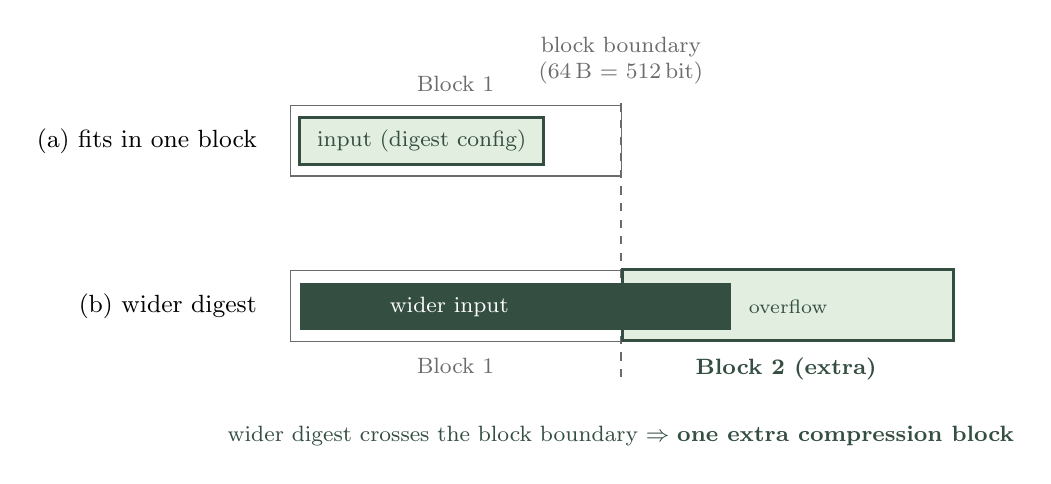
\begin{tikzpicture}[
  blk/.style={draw=reportgrey, minimum height=0.9cm, anchor=south west, font=\footnotesize},
  lbl/.style={font=\footnotesize, text=reportgrey},
  font=\small,
]

% geometry
\def\blkw{4.2}      % width of one compression block
\def\h{0.9}         % block height

% ============ ROW (a): fits in one block ============
\def\ya{2.4}
% Block 1 outline
\node[blk, minimum width=\blkw cm] (a1) at (0,\ya) {};
\node[lbl, anchor=south] at ({0.5*\blkw},{\ya+\h+0.06}) {Block 1};
% input bar fully inside block 1 (green)
\fill[reportsagetint, draw=reportsage, very thick]
  ({0.12},{\ya+0.15}) rectangle ({0.12+3.1},{\ya+\h-0.15});
\node[font=\footnotesize, text=reportsage] at ({0.12+1.55},{\ya+0.45}) {input (digest config)};
% row label
\node[anchor=east, font=\small, text=black] at (-0.3,{\ya+0.45})
  {(a) fits in one block};

% ============ block-boundary dashed line (64 B / 512 bit) ============
\def\yb{0.3}
\def\toplim{3.4}
\draw[dashed, reportgrey, thick]
  ({\blkw},{\yb-0.45}) -- ({\blkw},{\toplim});
\node[lbl, anchor=south, rotate=90] at ({\blkw+0.0},{\toplim+0.02}) {};
\node[lbl, align=center, anchor=south] at ({\blkw},{\toplim+0.05})
  {block boundary\\ (64\,B $=$ 512\,bit)};

% ============ ROW (b): wider digest spills over ============
% Block 1
\node[blk, minimum width=\blkw cm] (b1) at (0,\yb) {};
\node[lbl, anchor=north] at ({0.5*\blkw},{\yb-0.08}) {Block 1};
% Block 2 (extra) highlighted
\node[blk, minimum width=\blkw cm, fill=reportsagetint, draw=reportsage, very thick]
  (b2) at ({\blkw},\yb) {};
\node[text=reportsage, font=\footnotesize\bfseries, anchor=north]
  at ({1.5*\blkw},{\yb-0.08}) {Block 2 (extra)};
% input bar crossing the boundary
\fill[reportsage]
  ({0.12},{\yb+0.15}) rectangle ({\blkw+1.4},{\yb+\h-0.15});
\node[font=\footnotesize, text=white] at ({0.12+1.9},{\yb+0.45}) {wider input};
% overflow marker into block 2
\node[font=\scriptsize, text=reportsage, anchor=west]
  at ({\blkw+1.5},{\yb+0.45}) {overflow};
% row label
\node[anchor=east, font=\small, text=black] at (-0.3,{\yb+0.45})
  {(b) wider digest};

% ============ annotation under the whole thing ============
\node[align=center, font=\footnotesize, text=reportsage, anchor=north]
  at ({\blkw},{\yb-0.95})
  {wider digest crosses the block boundary $\Rightarrow$ \textbf{one extra compression block}};

\end{tikzpicture}
\end{document}
